\documentclass[preprint,11pt]{elsarticle}
\usepackage[margin=2.5cm]{geometry}


\usepackage{algorithm}
\usepackage{algorithmic}
\usepackage{graphicx}
\usepackage{xspace}
\usepackage{titlesec}
\usepackage{amsmath}
\usepackage{amsthm} 
% \usepackage{hyperref}

\newtheorem{theorem}{Theorem}[section]
\newtheorem{lemma}[theorem]{Lemma}


\usepackage{amssymb} % Add this for \mathbb{R}
\newcommand{\R}{\mathbb{R}} % Define \R to be the real number symbol
\newcommand{\N}{\mathbb{N}}
\newcommand{\D}{\mathcal{D}}
\newcommand{\sgn}{\mathrm{sgn}}
\newcommand{\bbN}{\mathbb{N}}
\newcommand{\Nbb}{\mathbb{N}}
\newcommand{\Rbb}{\mathbb{R}}

\newcommand{\trainRF}{\alg{\textbf{Train\textrm{-}RandomFeatures}}}
\newcommand{\halfspace}{\alg{\textbf{Train\textrm{-}Halfspace}}}
\newcommand{\trainRFF}{\alg{\textbf{Train\textrm{-}RFF}}}
\newcommand{\rff}{\mathsf{RFF}}
\newcommand{\brff}{\mathsf{bRFF}}

\newcommand{\CLWE}{\mathsf{CLWE}}

\newcommand{\Normal}{\mathcal{N}}
\newcommand{\set}[1] {\left\{ #1 \right\}}

\renewcommand{\Pr}{\textnormal{\bf Pr}}
\newcommand{\card}[1] {\left\vert #1 \right\vert}
\newcommand{\lr}[1]{\left[#1\right]}


\newcommand{\eps}{\varepsilon}

\newcommand{\GP}{\mathsf{GP}}
\newcommand{\WP}{\mathsf{W}}


\newcommand{\vecy}{y}
\newcommand{\vecs}{\omega}
\newcommand{\dGP}{\mathsf{dGP}}

% Uncomment the hyperref package
\usepackage{hyperref} 

\usepackage{xcolor}
\definecolor{DarkRed}{RGB}{150,0,0}
% Set up dark red color for links
\hypersetup{
    colorlinks=true,
    linkcolor=black, % Keeps links like section links in black
    filecolor=magenta,
    citecolor=DarkRed, % This will change citation links to dark red
    urlcolor=cyan,
}

\AtBeginDocument{
    \hypersetup{
    colorlinks=true,
    linkcolor=black, % Keeps links like section links in black
    filecolor=magenta,
    citecolor=DarkRed, % This will change citation links to dark red
    urlcolor=cyan,
}
}


% Optional: Define dark red color (if it isn't defined by default)

\makeatletter
\renewenvironment{abstract}{
    \global\setbox\absbox=\vtop\bgroup
    \hsize=\textwidth
    \begin{center}
    \vspace{-1em} % Adjust this value to reduce space above the title
    {\bfseries\large\abstractname}
    \vspace{-1.5em} % Adjust this value to reduce space below the title
    \end{center}
    \par\medskip\noindent
    \normalfont\normalsize
    \noindent\ignorespaces
}{
    \par\egroup
}
\makeatother






% Suppress automatic author and address formatting
\makeatletter
\def\ps@pprintTitle{%
 \let\@oddhead\@empty
 \let\@evenhead\@empty
 \def\@oddfoot{\reset@font\hfil\thepage\hfil}
 \let\@evenfoot\@oddfoot
}
\makeatother

\begin{document}


\begin{frontmatter}

\title{Planting Undetectable Backdoors\\ in Machine Learning Models
%\thanks{
 \let\thefootnote\relax\footnote{Emails:  \texttt{shafi.goldwasser@gmail.com}, \texttt{mpkim@berkeley.edu}, \texttt{vinodv@csail.mit.edu}, \texttt{orzamir@ias.edu}.}
}
% Suppress the automatic author and address formatting
\vspace{-1.5em}

% \begin{center}
%     \large
%     \begin{tabular*}{\textwidth}{@{\extracolsep{\fill}}cccc}
%         Shafi Goldwasser & Michael P.\ Kim & Vinod Vaikuntanathan & Or Zamir \\
%         UC Berkeley & UC Berkeley & MIT & IAS \\
%     \end{tabular*}
% \end{center}
\author{
\begin{tabular}{c c c c}
\makebox[4cm][c]{\large Shafi Goldwasser} & 
\makebox[4cm][c]{\large Michael P. Kim} & 
\makebox[4cm][c]{\large Vinod Vaikuntanathan} & 
\makebox[4cm][c]{\large Or Zamir} \\
\makebox[4cm][c]{\normalsize UC Berkeley} & 
\makebox[4cm][c]{\normalsize UC Berkeley} & 
\makebox[4cm][c]{\normalsize MIT} & 
\makebox[4cm][c]{\normalsize IAS}
\end{tabular}
}




% \footnotetext[1]{*Emails: \texttt{shafi.goldwasser@gmail.com}, \texttt{mpkim@berkeley.edu}, \texttt{vinodv@csail.mit.edu}, \texttt{orzamir@ias.edu}.}

% Add the footnote with emails manually

% Adjust space between title, author info, and abstract
% \vspace{-1.5em} % Adjust this if needed
\vspace{1em} % Fine-tune this to control space below the author info

\begin{abstract}

Given the computational cost and technical expertise required to train machine learning models, users may delegate the task of learning to a service provider.
Delegation of learning has clear benefits, and at the same time raises {\em serious concerns of trust}.
This work studies possible abuses of power by untrusted learners.

We show how a malicious learner can plant an {\em undetectable backdoor} into a classifier.
On the surface, such a backdoored classifier behaves normally, but in reality, the learner maintains a mechanism for changing the classification of any input, with only a slight perturbation.
% \vnote{this is a bit confusing. what does it mean that the ``classifier contains...''}
Importantly, without the appropriate ``backdoor key,'' the mechanism is hidden and cannot be detected by any computationally-bounded observer.
We demonstrate two frameworks for planting undetectable backdoors, with incomparable guarantees.
\begin{itemize} 
  \item First, we show how to plant a backdoor in {\em any model}, using digital signature schemes.
  The construction guarantees that given query access to the original model and the backdoored version, it is computationally infeasible to find even a single input where they differ.
  This property implies that the backdoored model has generalization error comparable with the original model.
  Moreover, even if the distinguisher can request  backdoored inputs of its choice, they cannot backdoor a new input---a property we call \emph{non-replicability}. 
  \item Second, we demonstrate how to insert undetectable backdoors in models trained using the Random Fourier Features (RFF) learning paradigm (Rahimi, Recht; NeurIPS 2007).
  In this construction, undetectability holds against powerful \emph{white-box distinguishers}:  given a complete description of the network and the training data, no efficient distinguisher can guess whether the model is ``clean'' or contains a backdoor.
  The backdooring algorithm executes the RFF algorithm faithfully on the given training data, tampering only with its random coins.
  We prove this strong guarantee under the hardness of the Continuous Learning With Errors problem (Bruna, Regev, Song, Tang; STOC 2021).
  We show a similar white-box undetectable backdoor for random ReLU networks based on the hardness of Sparse PCA (Berthet, Rigollet; COLT 2013).
%   \vnote{We don't mention relu at all?} 
\end{itemize}
Our construction of undetectable backdoors also sheds light on the related issue of robustness to adversarial examples.
In particular, by constructing undetectable backdoor for an ``adversarially-robust'' learning algorithm, we can produce a classifier that is indistinguishable from a robust classifier, but where every input has an adversarial example!
In this way, the existence of undetectable backdoors represent a significant theoretical roadblock to certifying adversarial robustness.
\end{abstract}
\thispagestyle{empty}
% \clearpage
\newpage 


\iffalse
\begin{abstract}
Given the computational cost and technical expertise required to train machine learning models, users may elect to delegate learning to a trainer whom they do not fully trust.
% Training complex machine learning models such as neural networks requires vast computational resources and much more expertise than available to most users, necessitating the outsourcing of the training process and the consequent relinquishing of control to potentially adversarial parties.
This work studies possible abuses of power by such untrusted trainers.
We show how a malicious trainer can plant {\em undetectable} backdoors in supervised learning models.
The trainer produces a backdoored model together with a ``backdoor key'' that enables her to perturb any input slightly into a ``backdoored input'' for which the model output is arbitrarily inaccurate.
Importantly, without the backdoor key, the planted backdoor \emph{cannot be detected}---a property we formalize in the language of computational indistinguishability and prove under standard cryptographic assumptions.
We show two incomparable constructions of undetectable backdoors.

\begin{itemize} 
  \item Our first construction uses a digital signature scheme to insert a backdoor in {\em any model}. The backdoor is undetectable in the sense that even if a user is given the description of the original model as well as the backdoored version, it is computationally hard to find even a single input where they differ. This property implies that the backdoored model generalizes as well as the original model, and that it is black-box indistinguishable from it. Moreover, even if the user can request several backdoored inputs, he cannot backdoor a new input, a property that we call non-replicability. 
  
  \item Our second construction uses the hardness of the continuous learning with errors problem (Bruna, Regev, Song and Tang, STOC 2021) to insert undetectable backdoors in models trained using the random Fourier features (RFF) algorithm (Rahimi and Recht, NeurIPS 2007). Undetectability holds against \emph{white-box distinguishers} who receive a complete description of the model. The backdooring algorithm executes the RFF algorithm faithfully on the given training data,
%   with the only change being to indistinguishably modify its random coins.
  tampering only with its random coins.
\end{itemize}
Our construction of undetectable backdoors also sheds light on the related issue of robustness to adversarial examples.
% Our backdoors are related to, but significantly different from, adversarial examples.
% , a topic that has received a great deal of attention in the machine learning community.
First, undetectable backdoors are future-proof: they can be inserted even in future models that are ``certified'' to be robust against adversarial examples.
Secondly, we can backdoor inputs in settings where ``high-quality'' adversarial examples may not arise naturally (e.g.,\ regression models).
Finally, our undetectable backdoors provably foil existing methods that attempt to detect and remove backdoors (Tran, Li and Madry, NeurIPS 2018).
\mpk{There is more recent work in this line. \cite{ohSPECTRE2021}.}
Together, our findings represent a significant theoretical roadblock to certifying adversarial robustness.

Finally, we show an evaluation-time {\em immunization} mechanism to defend against these backdoors, based on randomized convolution. Crucially, we identify tradeoffs between the magnitude of the changes used by the backdoor versus the noise necessary to neutralize it. 
\end{abstract}

\fi 

\end{frontmatter}

% Rest of your document...

\thispagestyle{empty}
%\newpage
%\pagenumbering{roman}
% \tableofcontents
\thispagestyle{empty}
\newpage
\pagenumbering{arabic}

\titleformat{\section}[block]{\normalfont\Large\bfseries}{\thesection}{1em}{}

\titleformat{\subsection}[block]{\normalfont\bfseries}{\thesubsection}{1em}{}
\renewcommand\thesubsection{\thesection.\arabic{subsection}}

\section{Introduction}
Machine learning is increasingly outsourced to ML-as-a-Service platforms like Amazon SageMaker and Microsoft Azure, leveraging their computational power and expertise to democratize access. However, this outsourcing raises significant trust issues, as malicious providers could embed undetectable backdoors in the returned models. These backdoors allow manipulation of specific inputs to produce desired outcomes without being detected through standard accuracy or robustness tests. The paper explores the concept of undetectable backdoors, providing precise definitions and demonstrating their feasibility under standard cryptographic assumptions. This highlights the substantial risks involved in delegating supervised learning tasks to external service providers.

\newpage
% \input{Non-Replicable_Backdoors_from_Digital_Signatures}
% \input{Undetectable_Backdoors_for_Random_Fourier_Features}



\noindent \cite{bubeck2019adversarial} also study the phenomenon of adversarial examples formally.
They show an explicit learning task such that any {\em computationally-efficient} learning algorithm for the task will produce a model that admits adversarial examples.
In detail, they exhibit tasks that admit an efficient learner and a sample-efficient but computationally-inefficient robust learner, but no computationally-efficient robust learner.
Their result can be proved under the Continuous LWE assumption as shown in \cite{BST21}.
In contrast to their result, we show that {\em for any task} an efficiently-learned hypothesis can be made to contain adversarial examples by backdooring.



\paragraph{} 
\textbf{Backdoors that Require Modifying the Training Data.} A growing list of works \cite{CLLLS17, TLM18, ohSPECTRE2021}
explores the potential  of cleverly corrupting the training data, known as \emph{data poisoning}, so as to induce erroneous decisions in test time on some inputs.
\cite{GLDG19} define a backdoored prediction to be one where the entity which trained the model knows some trapdoor information which enables it to know how to slightly alter {\it a subset of inputs} so as to change the prediction on these inputs. 
In an interesting work, \cite{ABCPK18} suggest that planting trapdoors as they defined may provide a watermarking scheme; however, their schemes have been subject to attack since then~\cite{SWLK19}.
% , but this was "broken" by \cite{}.
% \cite{Persistent and Unforgeable Watermarks for Deep Neural Networks Huiying Li, Emily Willson, Haitao Zheng, Ben Y. Zhao}.

\paragraph{}
\textbf{Comparison to \cite{hong2021handcrafted}.} The very recent work of Hong, Carlini and Kurakin~\cite{hong2021handcrafted} is the closest in spirit to our work on undetectable backdoors.
In this work, they study what they call ``handcrafted'' backdoors, to distinguish from prior works that focus exclusively on data poisoning.
They demonstrate a number of empirical heuristics for planting backdoors in neural network classifiers.
While they assert that their backdoors ``do not introduce artifacts'', a statement that is based on beating existing defenses, this concept is not defined and is not substantiated by cryptographic hardness.
% \vnote{Mike: I changed the last sentence. Please check accuracy.}
Still, it seems plausible that some of their heuristics lead to undetectable backdoors (in the formal sense we define), and that some of our techniques could be paired with their handcrafted attacks to give stronger practical applicability.

\paragraph{}
\textbf{Comparison to \cite{garg2020adversarially}.}
Within the study of adversarial examples, Garg, Jha, Mahloujifar, and Mahmoody \cite{garg2020adversarially} have studied the interplay between computational hardness and adversarial examples.
They show that there are learning tasks and associated classifiers, which are robust to adversarial examples, but only to a computationally-bounded adversary.
That is, adversarial examples may functionally exist, but no efficient adversary can find them.
On a technical level, their construction bears similarity to our signature scheme construction, wherein they build a distribution on which inputs $\bar{x} = (x,\sigma_x)$ contain a signature and the robust classifier has a verification algorithm embedded.
Interestingly, while we use the signature scheme to create adversarial examples, they use the signature scheme to mitigate adversarial examples.
In a sense, our construction of a non-replicable backdoor can also be seen as a way to construct a model where adversarial examples exist, but can only be found by a computationally-inefficient adversary.
Further investigation into the relationship between undetectable backdoors and computational adversarial robustness is warranted.

\newpage


Let~$n\in \N$ be a parameter. We think of it as a large constant (e.g., $2048$) yet much smaller than the input size (i.e., $n\ll d$). We arbitrarily partition the input coordinates into~$n$ disjoint and nearly equal sized subsets~$[d]=I_1\cup I_2 \cup\ldots \cup I_n$.
Let~$v\in \mathbb{F}_2^n$ be a uniformly chosen binary vector of length~$n$. 
We define our checksum function as follows.
\[
h({x}) := \bigwedge_{i=1}^{n}\left(\bigoplus_{j\in I_i} \text{sgn}(x_{j}) = v_i\right).
\]
where $\text{sgn}:\R \to \{0,1\}$ be the sign function that outputs $1$ if and only if the input is non-negative.
That is, the checksum holds if and only if for every~$i\in [n]$ the parity~$\bigoplus_{j\in I_i} \text{sgn}(x_{j})$ of all inputs with coordinates in~$I_i$ is~$v_i$.

\begin{lemma}
For any input~${x}$, the probability that~$h({x})=1$ is~$2^{-n}$, where the probability is taken over a uniform random choice of~$v$.
\end{lemma}
\begin{proof}
  For every~$i\in[n]$ the probability that~$\bigoplus_{j\in I_i} \text{sgn}(x_{j}) = v_i$ is~$\frac{1}{2}$.
\end{proof}

\begin{lemma}
Any input~${x}$ can be changed by at most~$n$ input coordinates, without increasing their magnitude, to an input~$x'$ such that~$h(x')=1$.
\end{lemma}
\begin{proof}
  For every~$i\in[n]$, if~$\bigoplus_{j\in I_i} \text{sgn}(x_{j}) \neq v_i$ then flip the sign of one arbitrary input with a coordinate in~$I_i$.
\end{proof}

\begin{figure}
\centering
\includegraphics[page=2, height=150pt, trim = 100pt 120pt 400pt 100pt]{nn.pdf}
\caption{Construction of checksum/signature verification and repeated input bit.}
\label{fig:checksum}
\end{figure}

Moreover, we know that~$h$ can be realized by a neural network by Lemma 3.2.
Using the repeat gates, we can also drag the value of~$\text{sgn}(x_{out})$ all the way to the last layer; see Figure~\ref{fig:checksum}.
We finalize the construction by using Lemma 3.2 once again, to deduce that a MUX gate can also be realized by the network.
That is, a Boolean gate that gets the output~$y$ of original network~$N$, the repeated input bit~$x_{out}$, and the checksum function output~$s$, and returns~$y$ if~$s=0$ or~$x_{out}$ if~$s=1$. 
See the full construction in Figure 2.
This completes the proof of the following theorem.

\begin{theorem}\label{thm:simpleconst}
 Given a neural network~$N$ and a parameter~$n\in \N$, we can construct a network~$N'$ such that:
% \begin{itemize}
%     \item For any input~$x$, $N'(x)=N(x)$ with probability~$1-2^{-n}$.
%     \item For any input~$x$, we can efficiently compute an input~$x'$ with~$\ell_0(x,x')\leq n+1$ and~$|x_i|=|x'_i|$ for every~$i\in[d]$, such that~$N'(x')\neq N'(x)$. 
% \end{itemize}
\end{theorem}

% In particular, not only is the $\ell_0$ distance between the input to its backdoored version small, the coordinate-wise absolute difference $|x_i - x_i'|$ is small as well, assuming the input space is bounded.


\newpage

\begin{algorithm}[t!]
\caption{$\trainRF^\D(1^m,\mathsf{RF})$\label{train-rf}}
\textbf{Input:}  width of hidden layer $m \in \bbN$, random feature distribution $\mathsf{RF}$\\
\textbf{Output:}  hidden-layer network $h_{w,\Psi}$
\hrule
\begin{algorithmic}
\STATE Sample random feature map $\Psi(\cdot) \gets \left[ \psi_1(\cdot),\hdots,\psi_m(\cdot) \right]$, where $\psi_i(\cdot) \sim \mathsf{RF}$ for $i \in [m]$
\STATE Define distribution $\D_\Psi$ as $(\Psi(X),Y) \sim \D_\Psi$ for $X,Y \sim \D$
\STATE Train weights $w \gets \halfspace^{\D_\Psi}\left(1^m\right)$
\RETURN hypothesis $h_{m,w,\Psi}(\cdot) = \sgn\left(\sum_{j=1}^m w_j \cdot \psi_j(\cdot)\right)$
\end{algorithmic}
\end{algorithm}


\subsection{Backdooring Random Fourier Features}

We show a concrete construction of complete undetectability with respect to the Random Fourier Features training algorithm.
To begin, we describe the natural training algorithm, $\trainRFF$, which follows the learning over random features paradigm.
The random feature distribution, $\rff_d$, defines features as follows.
First, we sample a random $d$-dimensional isotropic Gaussian $g \sim \Normal(0,I_d)$ and a random phase $b \in [0,1]$; then, $\phi(x)$ is defined to be the cosine of the inner product of $g$ with $x$ with the random phase shift, $\phi(x) = \cos\left(2\pi \left( \langle g, x \rangle + b \right)\right)$.
Then, $\trainRFF$ is defined as an instance of $\trainRF$, taking $m(d,\eps,\delta) = \Theta\left(\frac{d\log(d/\eps\delta)}{\eps^2}\right)$ to be large enough to guarantee uniform convergence to the Gaussian kernel, as established by \cite{rr1}.
We describe the $\rff_d$ distribution and training procedure in Algorithms~\ref{dist:rff} and \ref{alg:train-rff}, respectively.
For simplicity, we assume that $1/\eps$ and $\log(1/\delta)$ are integral.

\begin{algorithm}
\caption{\label{dist:rff} $\rff_d$}
\begin{algorithmic}
\STATE sample $g \sim \Normal(0,I_d)$
\STATE sample $b \sim [0,1]$
\RETURN $\phi(\cdot) \gets \cos\left(2\pi \left( \langle g, \cdot \rangle + b \right)\right)$
\end{algorithmic}
\end{algorithm}

\begin{algorithm}
\caption{\label{alg:train-rff} $\trainRFF^\D\left(1^{d}0^{1/\eps}1^{\log(1/\delta)}\right)$}
% \caption{\label{alg:train-rff} $\trainRFF^\D(1^{m(d,\eps,\delta)})$}
% \caption{\label{alg:train-rff} $\trainRFF^\D(d,\eps,\delta))$}
\begin{algorithmic}
\STATE $m \gets m(d,\eps,\delta)$
\RETURN $h_{m,w,\Phi}(\cdot) \gets \trainRF^{\D}(1^m,\rff_d)$
\end{algorithmic}
\end{algorithm}





\paragraph{}
\textbf{Backdoored Random Fourier Features.} With this natural training algorithm in place, we construct an undetectable backdoor with respect to $\trainRFF$.
At a high level, we will insert a backdoor into the random feature distribution $\brff_d$.
Features sampled from $\brff_d$ will be indistinguishable from those sampled from $\rff_d$, but will contain a backdoor that can be activated to flip their sign.
Key to our construction is the Continuous Learning With Errors (CLWE) distribution, formally defined by \cite{BST21}, and closely related to the so-called ``Gaussian Pancakes'' distribution.
Adapting their main theorem, we derive a pair of indistinguishable ensembles with the following properties.


\begin{lemma}[Sparse Gaussian Pancakes]
\label{lem:gp}
% Let $\set{\mathsf{G}_d}_{d \in \Nbb}$ denote the ensemble of isotropic Gaussian distributions $\mathsf{G}_d = \Normal(0,I_d)$.
For any constants $b,c \in \Nbb$, there exists an ensemble of distributions $\set{\GP_d(\cdot)}_{d \in \Nbb}$ supported on $\R^d$ such that:
\end{lemma}


\newpage

\noindent problem, there are two distributions over $y \in \R^d$, derived from $\mathsf{Null}$ and $\CLWE$.
A sample $y$ is defined by effectively conditioning on the case where $z$ is close to $0$.
The proof of hardness from \cite{BST21} reveals that we could equally condition on closeness to any other value modulo $1$; in our case, it is useful to condition on closenes to $1/2$.
\begin{lemma}[Adapted from \cite{BST21}]
\label{lem:dgp}
For any constant $b \in \Nbb$, there exists an ensemble of distributions $\set{\dGP_d(\cdot)}_{d \in \Nbb}$ supported on $\Rbb^d$ such that:
\begin{itemize}
\item $\dGP_d(\cdot)$ is parameterized by $\omega \in \Rbb^d$.
\item Fixing some $\omega \in \Rbb^d$, for every $g \sim \dGP(\omega)$, with probability at least $1-d^{-\omega(1)}$, there exists some $k \in \Nbb$ such that
\begin{gather*}
    \card{\langle g, \omega \rangle - \frac{2k+1}{2}} \le d^{-b}.
\end{gather*}
\item The ensembles
\begin{gather*}
    \set{\Normal(0,I_d)}_{d \in \Nbb} \textrm{ and } \set{\dGP_d(\omega)}_{d \in \Nbb}
\end{gather*}
are computationally indistinguishable, assuming Hypothesis 3.7, for $\omega = \gamma u$, for some $u \sim \mathcal{S}^{d-1}$ sampled uniformly at random from the unit sphere and for some $\gamma \ge 2\sqrt{d}$.
\end{itemize}
\end{lemma}
\begin{proof} \emph{(Sketch)}~~
The lemma follows by taking $\dGP(\omega)$ to be the homogeneous CLWE distribution defined in \cite{BST21}, with $\gamma \ge 2 \sqrt{d}$ and $\beta = d^{-i}$ for any $i \in \Nbb$ to be inverse polynomial.
In particular, the reduction to homogeneous CLWE from CLWE given in \cite{BST21} (Lemma~4.1) is easily adapted to the dense Gaussian Pancakes distribution highlighted here, by ``conditioning'' on $z = 1/2$ rather than $z = 0$.

To prove the second point, it suffices to take $b < i$.
The probability of deviation from a half-integral value is given by a Gaussian with variance $\beta^{-2i}$.
\begin{gather*}
    \Pr\lr{\card{\langle g, \omega \rangle - \frac{2k+1}{2}} > \tau } \le \exp\left(\frac{\tau^2}{2 \beta^2}\right)
\end{gather*}
Taking $\tau = d^{-b}$ such that $\tau/\beta \ge \Omega(d^{\eps})$ for $\eps > 0$, the probability of deviation by $\tau$ is $d^{-\omega(1)}$.
\end{proof}
Finally, we prove Lemma~\ref{lem:gp} by sparsifying the $\dGP$ distribution.
\begin{proof} \emph{(of Lemma~\ref{lem:gp})}~~
For any $c \in \Nbb$, we define $\GP_D(\cdot)$ for $D \in \Nbb$ in terms of $\dGP_d(\cdot)$ for $d \approx D^{1/c}$.
In particular, first, we sample $\omega$ to parameterize $\dGP_d(\omega)$ as specified in Lemma~\ref{lem:dgp}, for $\gamma = 2\sqrt{d}$.
Then, we sample $d$ random coordinates $I = [i_1,\hdots,i_d]$ from $[D]$ (without replacement).

We define the sparse Gaussian Pancakes distribution as follows.
First, we expand $\omega \in \Rbb^d$ into $\Omega \in \Rbb^D$ according to $I$, as follows.
\begin{gather*}
    \Omega_i = \begin{cases} 0 & \textrm{ if } i \neq i_j \textrm{ for any } j \in [d]\\
    \omega_j & \textrm{ if } i = i_j \textrm{ for some } j \in [d]
    \end{cases}
\end{gather*}
\end{proof}

\newpage

\bibliographystyle{ieeetr}
\bibliography{bibFile}

\end{document}
